\documentclass[journal,10pt,twocolumn]{article}
\usepackage{graphicx, float}
\usepackage[margin=0.5in]{geometry}
\usepackage{amsmath, bm}
\usepackage{array}
\usepackage{booktabs}
\usepackage{xfrac}

\providecommand{\norm}[1]{\left\lVert#1\right\rVert}
\let\vec\mathbf
\newcommand{\myvec}[1]{\ensuremath{\begin{pmatrix}#1\end{pmatrix}}}
\newcommand{\mydet}[1]{\ensuremath{\begin{vmatrix}#1\end{vmatrix}}}

\title{\textbf{CHAPTER-10 \\ STRAIGHT LINES}}


\begin{document}
\maketitle
\section*{Excercise 10.2}

Q4. Passing through $(2,2\sqrt{3})$ and inclined with the x-axis at an angle of $75^\circ$.

\section*{\large Solution}

\begin{figure}[H]
\centering
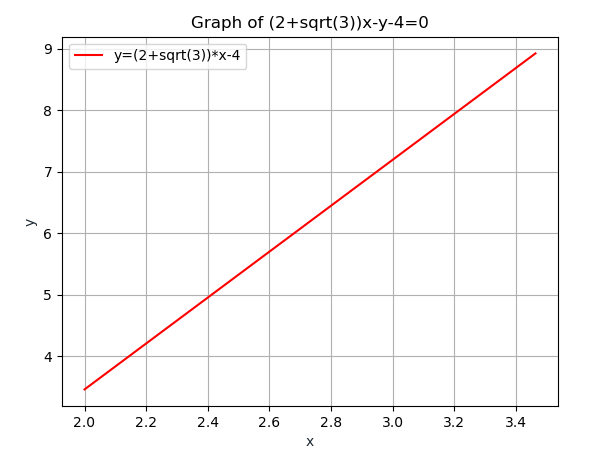
\includegraphics[width=1\columnwidth]{./figs/line.png}	
\caption{}
\end{figure}


\section{construction}

\begin{tabular}{|c|c|}
	\hline
	\textbf{Point}&\textbf{Value}\\
	\hline
	A&\myvec{2\\2\sqrt{3}}\\
	\hline
	$\theta$&75$^\circ$\\
	\hline
	
	
\end{tabular}


\section{Assumptions}
To find the line equation  through the point $\myvec{2\\2\sqrt{3}}$
\vspace*{3mm}

 The Directional vector is:

\begin{align}
\vec{m}=\myvec{1\\tan75^\circ}
	&=\myvec{1\\2+\sqrt{3}}
\end{align}
  
\section{Proof:}
we know that the Normal vector is:
\begin{align}
	\vec{n}&=\myvec{2+\sqrt{3}\\-1}\\
	\vec{n}^\top&=\myvec{2+\sqrt{3}&-1}	
\end{align}






Where line equation  is given by:
\begin{align}
	\vec{n}^\top \vec{{\vec{x}-\vec{A}}} &= 0
\end{align}

By substituting the values in the above equation:



\begin{align}
	\myvec{2+\sqrt{3} &-1}\vec{x}-\myvec{2\\2\sqrt{3}}&=0\\
	\myvec{2+\sqrt{3}&-1}\vec{x}&=4
\end{align}


\end{document}
